\chapter{Executive Summary}
The Oregon Department of Transportation (ODOT) has long been a leader in the development of statewide integrated transport-land use models. This document describes the functional form of their second generation model, named the StateWide Integrated Model (SWIM2). The SWIM2 system represents the behavior of the economy, land use, and transport system in the State of Oregon and the interactions between them. The system is composed of a set of interconnected components that simulate different aspects of the full system:

\begin{itemize}
\item The New Economics and Demographics (\textbf{NED}) component determines model-wide production activity levels, employment, and imports and exports based upon official Oregon state forecasts.
\item The two-stage Synthetic Population Generator (\textbf{SPG}) component samples household and person demographic attributes (SPG1) and assigns a household to an alpha zone (SPG2).
\item The Aggregate Land Development (\textbf{ALD}) component allocates model-wide land development decisions among study area zones considering floorspace prices and vacancy rates.
\item The Activity Allocation (\textbf{AA}) component determines commodity (goods, services, floorspace, labor) quantity and price in all exchange zones to clear markets, including the location of business and households by beta zone.
\item The Person Travel (\textbf{PT}) component generates activity-based person trips for each study area person in the synthetic population during a typical weekday, and assigns a workplace alpha zone.
\item The Commercial Transport (\textbf{CT}) component generates mode split for goods movement flows and generates truck trips, combining shipments and possible trans-shipment locations, for a typical weekday.
\item The External Transport (\textbf{ET}) component generates truck trips from through movements based on external station growth rates.
\item The Transport Supply (\textbf{TS}) component assigns vehicle, truck, and transit trips to paths on the congested transport network for a 24-hour period, generating time and distance skims for AM and off-peak periods.
\end{itemize}

\noindent The structure of the overall model is shown in Figure \ref{fig:tlumip-schematic}. The model steps through time in one-year intervals, typically to a forecast horizon in the year 2030. The system also includes two optional components:
\begin{itemize}
\item The Economic Feedback (\textbf{EF}) component is a simplified dynamic feedback to that adjusts the fixed modelwide economic forecast generated by NED, considering the statewide composite location utilities by industry from the AA component. This functionality is in place, but has not been extensively tested. 
\item The Select Link (\textbf{SL}) component generates SWIM2 highway assignment paths for later use in generating outputs such as select link results, subarea matrices, and route choice results.\footnote{AA currently assigns the trip tables in the CT, ET, and PT modules using VISUM installed on the TLUMIP computer cluster.}
\end{itemize} 

\begin{figure}  % Figure 1.1, trim=l b r t
\centering
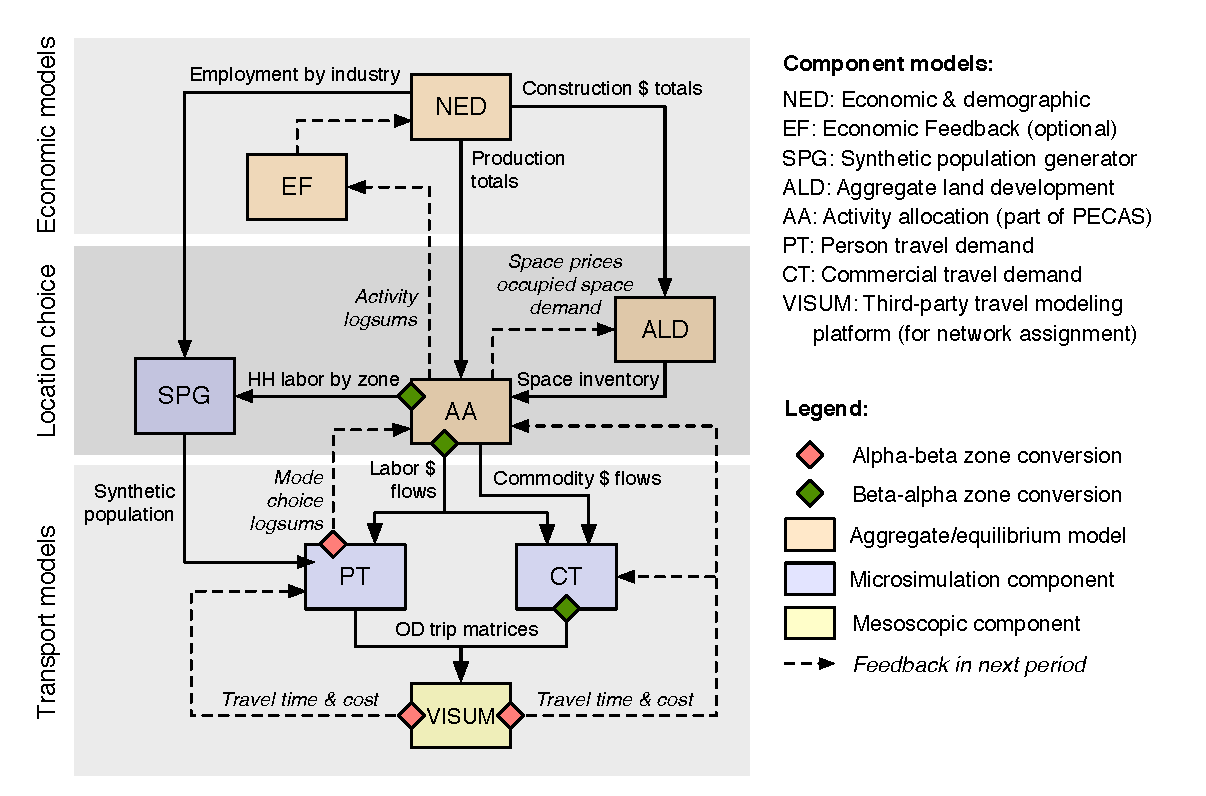
\includegraphics[scale=0.75, trim=1mm 1mm 1mm 1mm, clip]{summary/swim25-schematic}  
\caption{Modules and flows in the second generation Oregon StateWide Integrated Model (SWIM2)}
\label{fig:tlumip-schematic}
\end{figure}

\noindent The basic functionality of the SWIM2 system has been calibrated using several approaches:
\begin{itemize}
\item A three-stage approach to the calibration of the model has been implemented. The various parameters in each module have been sorted into three categories (S1, S2, and S3), related to the three stages in the calibration when they are considered.
\item Real-world (observed) values for more than 20 module outputs were established and used as targets for completing the S2 (each modules in isolation) and initial S3 (full model) calibration.
\item Calibration for a 1998 base year and trends over time was completed and shared with the TLUMIP Peer Review Panel in June 2008. The CT and PT modules have undergone further updates and were re-calibrated in October 2010. The NED and AA components (replacing the original ED and PI modules) were updated, and the spatial models re-calibrated in August 2011.  
\end{itemize}

\noindent The following user interface improvements have been made to support the use of the SWIM2 system:
\begin{itemize}
\item Implementation of a Model Runner System Graphical User Interface (MrsGUI) for facilitating model use, such as scenario creation, starting and monitoring model runs, and facilitating scenario archiving.
\item Implementation of a database (VIZ DB and VIZ DB Micro) to house model zone, link and microsimulation outputs in standardized format, as well as a visualization tool (SWIMVIZ) that enables a user-friendly dynamic queries and visualization of the multi-year model output in maps and charts.
\item Maintenance of a SWIM2 User'��s Guide including instructions for installing and running the model on the ODOT State Data Center (SDC) computer cluster, as well as other user information and instructions.
\end{itemize}

\noindent With this document and associated software, the SWIM2 functionality has been finalized and calibrated, and is ready for policy application. The following activities were undertaken to reach this outcome:
\begin{itemize}
\item All modules are completed as documented in this Guide, including software and inputs.
\item Software was developed in order to implement the full modeling system as specified, as confirmed through testing and calibration.
\item The values for the all parameters for each module have been developed, with many estimated statistically.
\item Base year inputs for all modules have been developed or synthesized, including the auto and transit networks.
\end{itemize}

% Note the references in the following paragraph

\noindent The SWIM2 system has the following advantages over the first generation SWIM1 model, completed in 1999 and implemented in the TRANUS platform \citep{donnelly99}: 
\begin{itemize}
\item Endogenously-generated regional economic forecasts, based on exogenous national forecasts, using the NED module.
\item More comprehensive aggregate treatment of regional economic flows (AA module), including explicit representation of commodities separate from industries and explicit treatment of related exchange locations and exchange prices.
\item Separation of management (white-collar) and production (blue-collar) components of production activities and the associated separation of consumption of these activities.
\item Much greater number of economic sectors considered in the economic and activity allocation modules (38 sectors, plus 14 white-collar/light-heavy industry sub-sectors, compared to 12 in SWIM1), as well as two non-household institutions.
\item Consideration for significantly more goods commodities (39 compared to 12 in SWIM1), as well as services and labor occupations.
\item Much greater number of space categories considered in land development and in production and consumption activity allocation (18 categories compared to 2 in SWIM1).
\item More intuitive zoning input used in land development (ALD), with 31 zoning codes.
\item Micro-level simulation of population (SPG module).
\item Much greater number of household sectors considered in activity allocation (AA module), stratified by household size as well as income group (18 compared to 3 in SWIM1).
\item Microsimulation of daily travel for nearly 6 million people within the study area (PT module).
\item Microsimulation of daily freight movements, including trans-shipment centers (CT module) and a wider range of vehicle types and related configurations.
\item Improved geographic coverage, including internal modeling of a roughly 50-mile halo region around the state of Oregon, which has as much activity as the state itself.
\item Significantly more detailed zones (2,950 alpha zones and 518 beta zones, compared to 125 zones in SWIM1) and networks (over 53,000 links, compared to nearly 2,000 in SWIM1).
\item Significantly higher temporal resolution options with time increments of one year, rather than five-year intervals in TRANUS.
\item Implementation of a distributed computing approach to help reduce run times for the SWIM2 modeling system.
\end{itemize}